\chapter{Analysis with Sample Dataset}
Having developed a framework to examine the models, attention was turned to some analyses that could be carried out within the time frame and scope of the project\footnote{Please refer to  \S\ref{chapt:RECOMMENDATIONS} for recommendations for further work}. With this in mind, it was decided to focus analysis on the a smaller subset of the training dataset, namely documents from the University of Cambridge Chemistry Department. This dataset is henceforth referred to as \emph{CCD}\footnote{Cambridge Chemistry Dataset}.
\section{Cambridge Chemistry research clusters}
\label{sec:RESEARCHCLUSTERS}
The CCD contained 9467 documents. The cosine matrix was calculated and a network was constructed from the matrix. \emph{Communities} within the network (clusters of strongly connected nodes) were identified by applying a high throughput modularity algorithm\cite{modularity1}\cite{modularity2}. The result is shown in figure \ref{fig:CAMCOMMUNITIES}.
\begin{center}
\begin{figure}[H]
  \centering
  \textbf{CCD Network Visualisation}
    \includegraphics[width=\textwidth]{Analysis/cam.png}
    \caption[Network Visualisation of University of Cambridge Chemistry Department Documents]{A Network visualisation of the CCD. Edges were placed between nodes with weights corresponding to cosine similarity if $S_{cosine}$. Nodes are coloured by their detected communities, and node size is proportional to the number of connections a node has. nodes are arranged by modelling edges as springs.}
    \label{fig:CAMCOMMUNITIES}

\end{figure} 
\end{center}
It is apparent that the CCD contains contains clear communities of documents. This corresponds to different fields of research within the department. Some communities detected were small, but some quite large (green, orange, etc...). The algorithm was then applied only to `green' community, which revealed subcommunities within the `green' documents. A program was then written to recursively detect subcommunities in the CCD. This resulted in the CCD being divided into 300 communities of comparable size. The smallest communities were singleton documents, the largest community was 434 documents, and the mean population was 34.5. The community finding subdivision process is shown in figure \ref{fig:COMMTREE}
\begin{center}
\begin{figure}[H]
  \centering
  \textbf{Recursion Tree for Community Generation Process}
    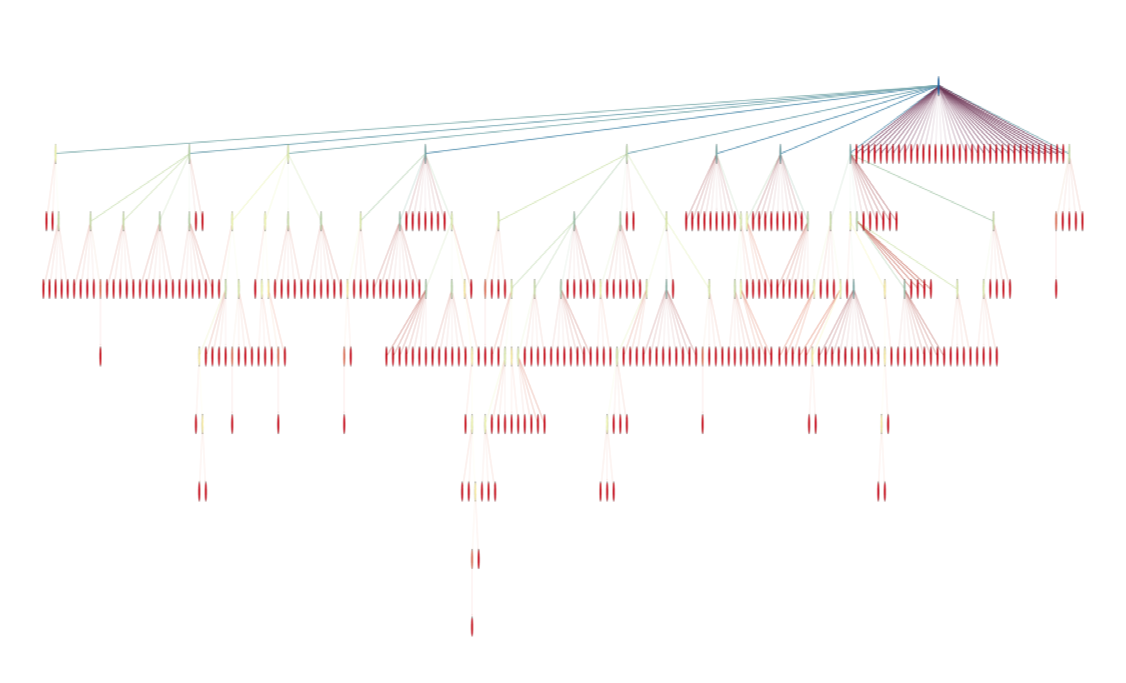
\includegraphics[width=\textwidth]{Analysis/comms.png}
    \caption[Recursion Tree for Document Community Generation]{Recursion Tree for how communities were derived. The dataset was partitioned using the modularity algorithm. Sets with more than 100 documents were then repartitioned recursively. Sets of less than 100 documents were considered to be communities (red nodes in the diagram). If the algorithm could not partition a set any further, the recursion was stopped and the set was considered a community, even if it was larger than 100 documents.  The figure shows the maximum depth of partitioning required was 8, and most communities were found after 3 partitions.}
    \label{fig:COMMTREE}

\end{figure} 
\end{center}
Figure \ref{fig:COMMTREE} can be interpreted as showing the \emph{relationships} between different fields of research within the department. The tree is shallow with highly branched nodes, suggesting wide research fields, and much qualitative overlap between fields.
The process described is constitutes an unsupervised categorisation algorithm. The entire process, from model training to finding communities has been performed without human labelling or intuition. It was therefore instructive to examine what the algorithm defined as communities.
Communities were examined closely, to reveal that community clustering made intuitive sense in the majority of cases. Community 275 is typical:
\begin{table}[H]
\centering
\caption{Community 275}
\label{tab:com275}
\begin{tabular}{||c|X||}
\hline
Community Size                   & 15                                                                                                                                                                 \\ \hline
Depth down Recursion Tree        & 2                                                                                                                                                                  \\ \hline
Contents                         & Bees, Neonicotinoids, toxicology, pollen.                                                                                                                          \\ \hline
Article closest to Mean Vector                      & 10.1021/es2035152: \footnotesize{Assessment of the Environmental Exposure of Honeybees to Particulate Matter Containing Neonicotinoid Insecticides Coming from Corn Coated Seeds} \\ \hline \hline
Community members                & (Some omitted for brevity)                                                                                                                                         \\ \hline
10.1007/s00216-012-6338-3        & \footnotesize{UHPLC-DAD  method for the determination of neonicotinoid insecticides in single bees and its relevance in honeybee colony loss investigations }                    \\ \hline
10.1021/es2035152                & \footnotesize{Assessment of the Environmental Exposure of Honeybees to Particulate Matter Containing Neonicotinoid Insecticides Coming from Corn Coated Seeds }                   \\ \hline
10.1007/s11356-014-3470-y        & \footnotesize{Systemic insecticides (neonicotinoids and fipronil): trends uses mode of action and metabolites                                                                   } \\ \hline
10.1111/j.1439-0418.2012.01718.x & \footnotesize{Aerial powdering of bees inside mobile cages and the extent of neonicotinoid cloud surrounding corn drillers}                                                       \\ \hline
10.1098/rsif.2013.0394           & \footnotesize{Analysing photonic structures in plants                                                } \\ \hline
10.1007/s00114-013-1020-y        & \footnotesize{The influence of pigmentation patterning on bumblebee foraging from flowers of Antirrhinum majus                                                                  } \\ \hline
10.1111/ics.12035                & \footnotesize{ Keratins and lipids in ethnic hair                                                                                                                                } \\ \hline
10.1021/ja047905n                & \footnotesize{Photoluminescent Layered Lanthanide Silicates                                                                                                                     } \\ \hline
\end{tabular}
\end{table}

Table \ref{tab:com275} shows that this particular research community refers mainly to toxicology studies of neonicotinoids,  bees and flowers\footnote{Note only some members of the community are shown above. Care was taken to give a representative sample of all 15 articles. The rest refer to Neonicotinoid insecticide studies with honey bees, and honey bee affinity to corn and pollen}. The connections mostly make sense. Note the surprising inclusion of the cosmetics and lanthanide silicate studies. Upon investigation, both studies use very similar analytical techniques used elsewhere in the community, and both examined intercalation.
\footnote{Both used made use of powder X-ray diffraction, and the silicates paper used thermogravimetry, the cosmetics study uses FID and several types of liquid chromatography, all methods used in the bee/neonicotinoid studies.}

Note also that the mean vector for the community was closest to a paper in the training set that summarised the community extremely well. This paper could be considered as a \emph{Summary paper.}
The uses of this kind of analysis include:
\begin{itemize}
\item Analysis of literature field - plotting trees such as figure \ref{fig:COMMTREE} can give a relational understanding of how facets of a field link up together. 
\item Research tool: If researching a paper, identifying its community immediately provides the researcher with papers that are related to it. Crucially this is done without simply following citations, so that interesting, perhaps overlooked links between papers can be found.
\item Summarising: If a researcher is required to read many papers from a field, they could find the communities involved and begin by reading the `summary' papers. 
\end{itemize}

\section{Cambridge Staff Member Similarities}
\label{sec:AUTHORCLUSTERS}

It is not only articles themselves that can be grouped and analysed, but articles can be aggregated together to represent higher order concepts, such as staff members or research groups, or potentially even departments. 

To investigate this further, \texttt{http://www.ch.cam.ac.uk/publications/authors} was scraped in order to associate the documents in the CCD with particular staff members. A staff member vector $\textbf{f}$ was defined as $\mathbf{f}=\frac{1}{N}\sum_{i}^{N} \mathbf{v}_i$ , for an author with $N$ published articles in the CCD, with document vectors $\mathbf{v}_i$ (vector mean).

To investigate author relationships, a cosine matrix was created for each pair of authors A and B, with $\alpha$ and $\beta$ documents respectively, $\mathbf{C^{\left( A \right ) , \left( B \right)}}$ (see \S\ref{sec:COSINEMAT}). The similarity between the author pair was defined as 
$$S_{A , B} = \sum_{i}^{\alpha} \sum_{j}^{\beta} C^{\left( A \right) , \left( B \right) }_{ i , j }$$
An \emph{author similarity matrix} can then be built up, $\mathbf{S}$, with elements $\mathbf{S}_{ A , B }=S_{ A , B }$.
A similar technique to that described in  \S\ref{sec:RESEARCHCLUSTERS} could have been used to create clusters of authors. Since the sample size was now much smaller (47 authors compared to 9467 papers) a more appropriate technique, Dedicated Hierarchical Clustering, specifically UPGMA \footnote{Unweighted Pair Group Method with Arithmetic Mean} was applied \cite{heatmapcluster}. This method clusters the authors pairwise in a hierarchical fashion.  An effective visualisation of the similarities between staff was to plot a \emph{clustermap} \cite{seaborn} \cite{scipy}.
\begin{center}
\begin{figure}[H]
  \centering
  \textbf{Cambridge Author Similarity Clustermap}
    \makebox[\textwidth][c]{\includegraphics[width=1.2\textwidth]{Analysis/authorsims.png}}
    \caption[Cambrdige Author Similarity Clustermap]{This figure shows a heatmap of author similarity. Dark pixels correspond to the author in the pixel's row having similar research interests to the author in the pixel's column. The matrix has been scaled to the range ($0 \rightarrow 1$).  The authors are arranged by clusters found in UPGMA. The hierarchical clustering structure is demonstrated by the dendrogram tree connecting author pairs together.}
    \label{fig:AUTHORSIMS}

\end{figure} 
\end{center}
Figure \ref{fig:AUTHORSIMS} shows the result of generating $\textbf{S}$ and performing UPGMA hierarchical clustering. The authors are labelled by crsid. The dendrogram tree links authors pair-by-pair, illustrating how the clustering was performed, and how closely related clusters are. An enlarged dendrogram is shown below:
\begin{center}
\begin{figure}[H]
  \centering
  \textbf{Cambridge Author Similarity Dendrogram}
    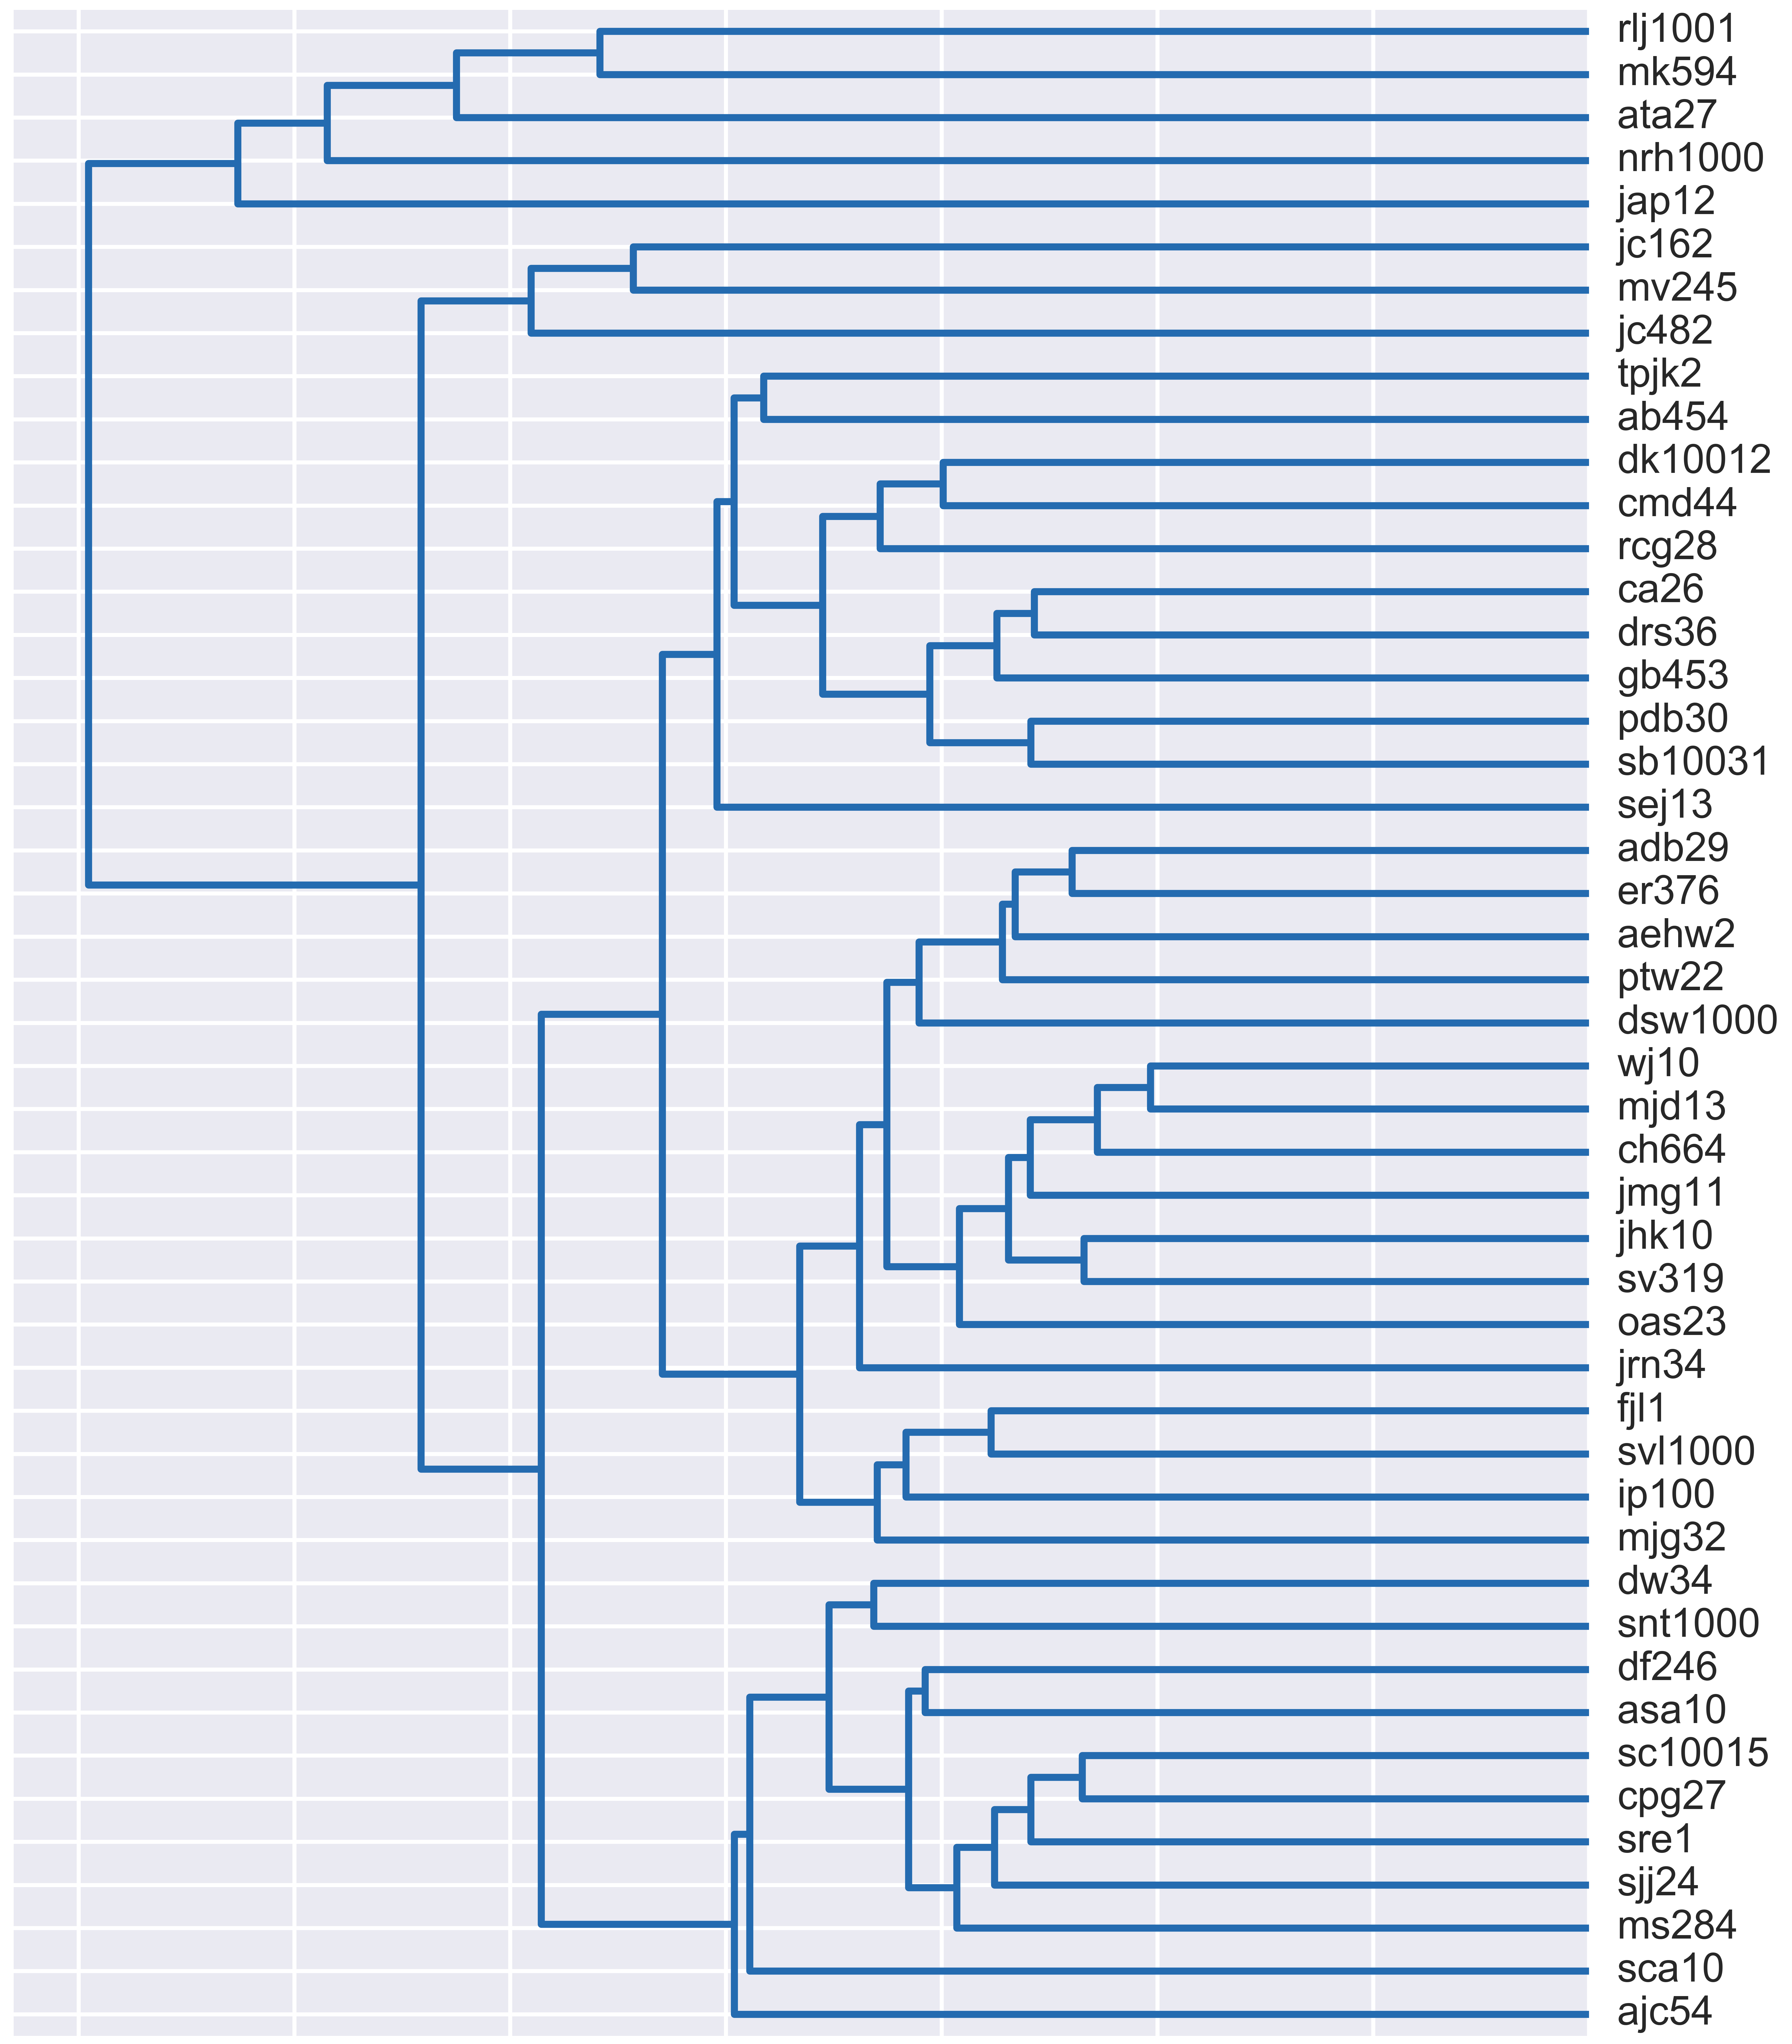
\includegraphics[width=\textwidth]{Analysis/dendro.png}
    \caption[Cambridge Author Similarity Dendrogram]{The dendrogram of figure \ref{fig:AUTHORSIMS}} plotted for clarity
\end{figure} 
\label{fig:DENDRO}

\end{center}
A striking feature of figure \ref{fig:AUTHORSIMS} is the cluster in the bottom right corner. The dendrogram tree shows the members of this cluster occupy a separate branch of research space than the rest of the department. The staff members involved (Professors Jones and Pyle, Drs. Harris, Archibald and Kalberer) are all members of the Centre for Atmospheric Science. The unsupervised model thus successfully `predicted' their department, and indicated that their work is quite separate from most of the work in the Chemistry Department. This is a real success for the model. The dendrogram was then further examined and broken into distinct branches. Each branch was examined and manually labelled (see figure \ref{fig:LABELLEDDENDRO}. Most clusters make intuitive sense, but there is one core of well connected, more disparate members (wj10 to jrn34). These members could be interpreted as forming an interdisciplinary cluster.  
\begin{center}
\begin{figure}[H]
  \centering
  \textbf{Annotated Dendrogram}
    \includegraphics[scale=0.8]{Analysis/dendro_overlay2.png}
    \caption[Dendrogram annotated with labelled fields]{Cluster labels overlayed over the distinct branches of the dendrogram.}
    \label{fig:LABELLEDDENDRO}
\end{figure} 
\end{center}
The value of this method is self evident. Clustering staff members informs the department about the width of research (number of clusters), and how resources are partitioned (size of clusters). It should also be stressed that authors are associated without any human preconceptions or bias. Thus perhaps the most valuable author associations are the unexpected ones, and authors should be encouraged to examine their cluster and consider their `neighbours'.
\section{Combining research clusters and authors}
As a final data examination, the topic communities found in  \S\ref{sec:RESEARCHCLUSTERS} were linked to the staff members. Different metrics for author similarity were developed to investigate if they correlated with the maps produced in \S\ref{sec:AUTHORCLUSTERS}.
Firstly, for a topic community $\mathfrak{C}$, with documents $d \in \mathfrak{C}$, and an author $\mathfrak{A}$ with documents $\delta \in \mathfrak{A}$, we can associate the author with the community if $\mathfrak{C} \cap \mathfrak{A} \neq \{ \}$, \footnote{or equivalently $\exists  \partial : \partial \in \mathfrak{C} \wedge \partial \in \mathfrak{A} $}. The function $f_{assoc}$ was defined as 
\[ 
f_{assoc}\left( \mathfrak{C} , \mathfrak{A} \right) = \begin{cases} 
      0 & \mathfrak{C} \cap \mathfrak{A} = \{ \} \\
      1 & \mathfrak{C} \cap \mathfrak{A} \neq \{ \} 
   \end{cases}
\]
It was noted that there was significant variation in the number of communities that researchers were associated with. A plot of $\sum_c^C f_{assoc} \left( \mathfrak{C}_c , \mathfrak{A} \right)$ for each author is shown below:
\begin{center}
\begin{figure}[H]
  \centering
  \textbf{Author Community Spread}
    \includegraphics[width=\textwidth]{Analysis/Community_detection_with_ordering.png}
    \caption[Author community Spread]{Number of research communities authors are associated with. High values (towards red) indicate an author publishing across many communities, suggest more interdisciplinary work, but also higher publication count per author. The authors are ordered by publication count (highest at top). As expected, there is a correlation between publication count and number of communities an author appears in. The blue dotted line-of-best-fit divided the authors into those that publish more widely given their publication count (Bar to the right of the line) form those who publish more narrowly for their publication count (Bar to the left of the line)}
\label{fig:commbar}

\end{figure} 
\end{center}
It can be seen that some authors are widely distributed between communities, whereas others are concentrated.
It should be appreciated that communities are not uniformly distributed. For example there are many communities in `Life Sciences' but few in Atmospheric Chemistry, as such, interpretation of high values in Figure \ref{fig:commbar} directly corresponding to wide research interests should be tentative\footnote{It should also be noted that figure \ref{fig:commbar} treats strong connects equally to weak connections, i.e. 100 papers published in one community is just as strong a connection to 1 paper published in a community}.

An association metric $S_{coincidence}$ between authors $\mathfrak{A}$ and $\mathfrak{B}$ was then defined as $$S_{coincidence}\left( \mathfrak{A} , \mathfrak{B} \right) = \sum_c^C \left(f_{assoc} \left( \mathfrak{C}_c , \mathfrak{A} \right) f_{assoc}\left( \mathfrak{C}_c , \mathfrak{B} \right) \right) $$
Where $C$ is the total number of communities. An association matrix was created, $\mathbf{S}^{Assoc}_{\mathfrak{A} , \mathfrak{B}} = S_{coincidence}\left( \mathfrak{A} , \mathfrak{B} \right)$, where high values for author pair $\mathfrak{A} , \mathfrak{B}$ indicate they appear in many research communities together. The matrix was then scaled such that: $\mathbf{S}^{Assoc,scaled}_{\mathfrak{A} , \mathfrak{B}} =  \mathbf{S}^{Assoc}_{\mathfrak{A} , \mathfrak{B}} /  \left( \mathbf{S}^{Assoc}_{\mathfrak{A} , \mathfrak{A}} + \mathbf{S}^{Assoc}_{\mathfrak{B} , \mathfrak{B}} \right) $, and scaled from $0 \rightarrow 1$. This was a measure of how often authors could be found in the same communities. The matrix is shown below:
\begin{center}
\begin{figure}[H]
  \centering
  \textbf{Author Coincidence Heatmap}
    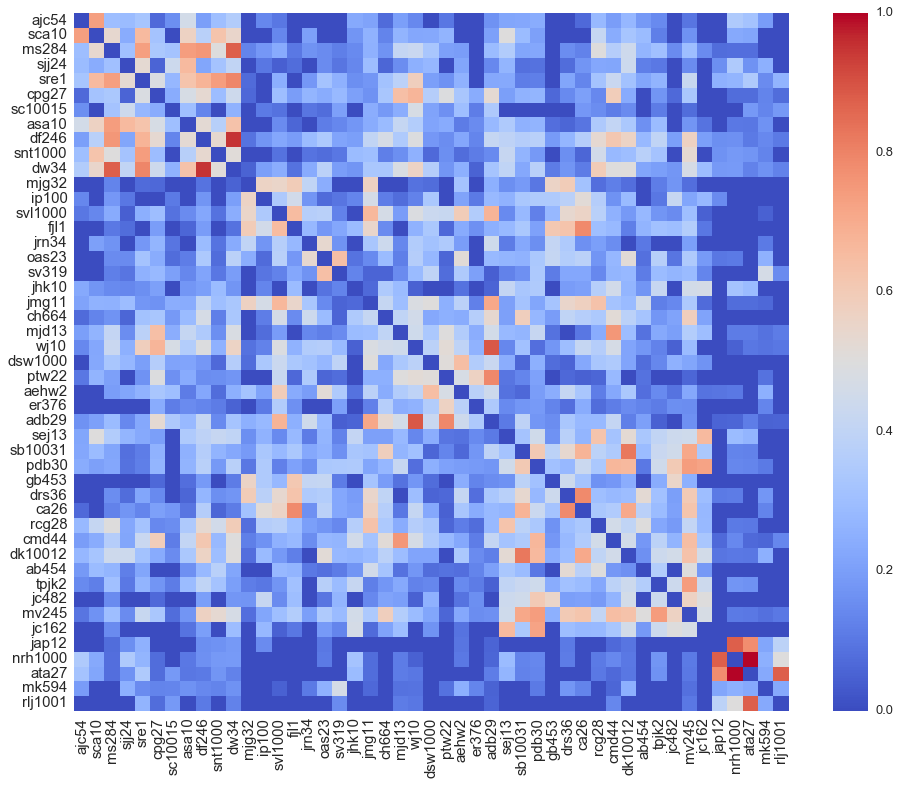
\includegraphics[width=\textwidth]{Analysis/author_comm_heatmap.png}
    \caption[Author Coincidence Matrix Heatmap]{Heatmap showing author-author pair values for how often author pairs publish works in the same communities. High values indicated that aduthors are predicted to have similar publication profiles. Note the authors are arranged with the ordering from figure \ref{fig:AUTHORSIMS}.}
    \label{fig:commHEATMAP}

\end{figure} 
\end{center}
Figure \ref{fig:commHEATMAP} displays where authors have been detected to have similar research community occupations. High values should indicate that authors should ideally collaborate/communicate because they publish in the same research communities. Note also that the square patterns of higher values close to the diagonal of the map reproduces the clustering in figure \ref{fig:AUTHORSIMS}, lending weight to the validity of both analyses.\footnote{This is because the heatmap has been arranged according to the clustering found in \S\ref{sec:AUTHORCLUSTERS}, but the matrix in figure \ref{fig:commHEATMAP} is derived with a completely different method (without applying any clustering algorithm to the authors). Because clustering is qualitatively visible in figure \ref{fig:commHEATMAP}, there is a correlation between the two methods, i.e. they are consistent}.

Having defined a framework for finding where authors share research interest, the next step was to find where authors were \emph{actually} collaborating. It was possible to identify approximately 700 documents in CCD that were co-authored by staff members in the analysis. A heatmap for actual collaboration between authors is shown below, as well as a metric equivalent to the $\mathbf{S}^{assoc,scaled}$ with elements as the sum of the number of communities both staff members have collaborated in.

\begin{figure}[H]
  \centering
  \textbf{Author Collaboration Heatmap}
    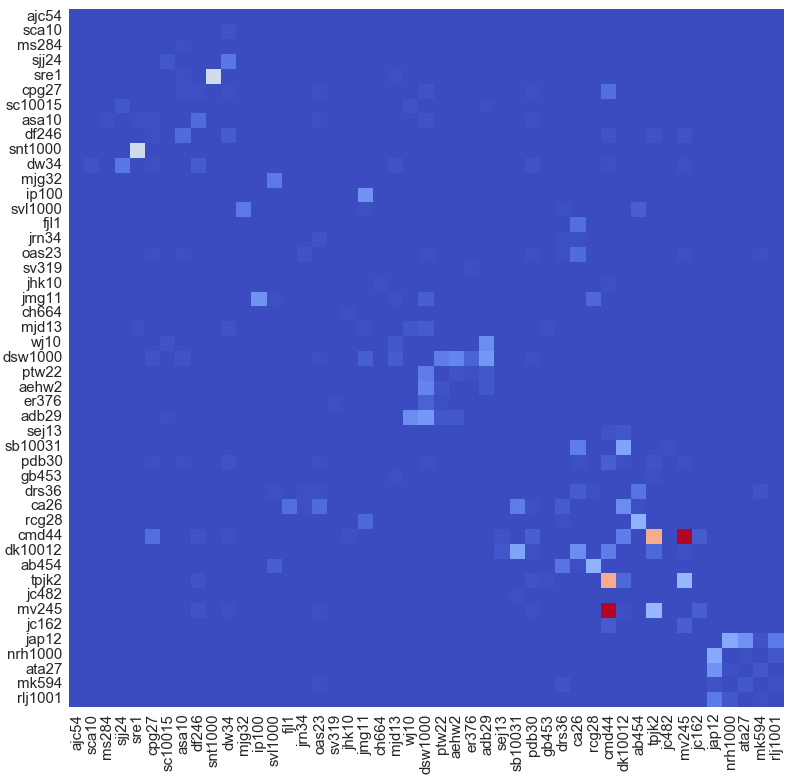
\includegraphics[width=\textwidth]{Analysis/raw_collabs.png}
    \caption[Author Collaboration Heatmap]{Raw collaboration matrix (values scaled to range $0 \rightarrow 1$). Note the general lack of co-publishing between staff members. Again staff are ordered by clustering described in \S\ref{sec:AUTHORCLUSTERS}, but no actual clustering has been performed. Hot spots near the diagonal suggest that author pairs clustered close together in \S\ref{sec:AUTHORCLUSTERS} generally collaborate more than distant author pairs.}
      \label{fig:rawcollabs}
  \end{figure}
  \begin{figure}
  \centering
  \textbf{Community-summed Author Collaboration Heatmap}
    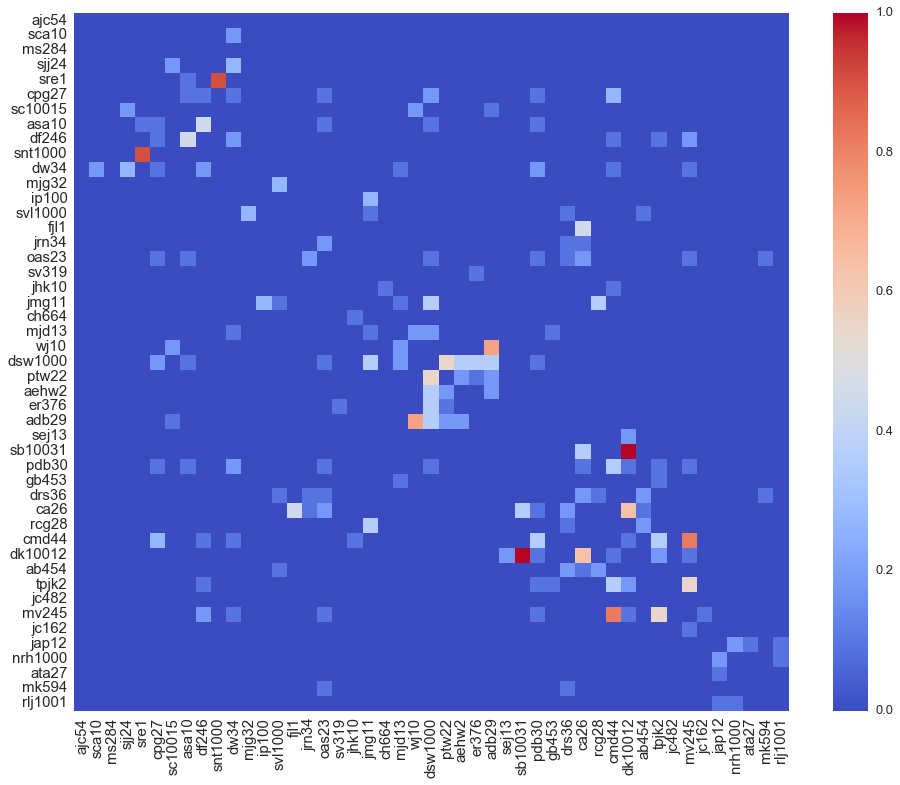
\includegraphics[width=\textwidth]{Analysis/comm_collabs.png}
    \caption[Community-summed Author Collaboration Heatmap]{Matrix formed by summing collaboration of author pairs over research communities (values scaled to range $0 \rightarrow 1$). Qualitatively similar to figure \ref{fig:rawcollabs}. Hot spots near diagonal again suggest authors closely clustered in \S\ref{sec:AUTHORCLUSTERS} collaborate more frequently }
      \label{fig:collcollabs}

\end{figure}

Both pictures show the same qualitative picture. Similar author pairs (close to diagonal) are more likely to collaborate. 

As a final data step, a matrix defined as the difference between an author similarity matrix (e.g figures \ref{fig:AUTHORSIMS}, \ref{fig:commHEATMAP}) and an author collaboration matrix (e.g. figures \ref{fig:rawcollabs}, \ref{fig:collcollabs}) could be interpreted as a \emph{recommended collaboration matrix}, i.e. where values close to 1 indicate high similarity but low evidence of collaboration, values close to 0 indicate effective collaboration and values close to -1 indicate high collaboration but low author similarity. Author Pairs with values to 1 should be encouraged consider working together. This matrix is shown below:
\begin{center}
\begin{figure}[H]
  \centering
  \textbf{Recommended Collaboration Matrix}
    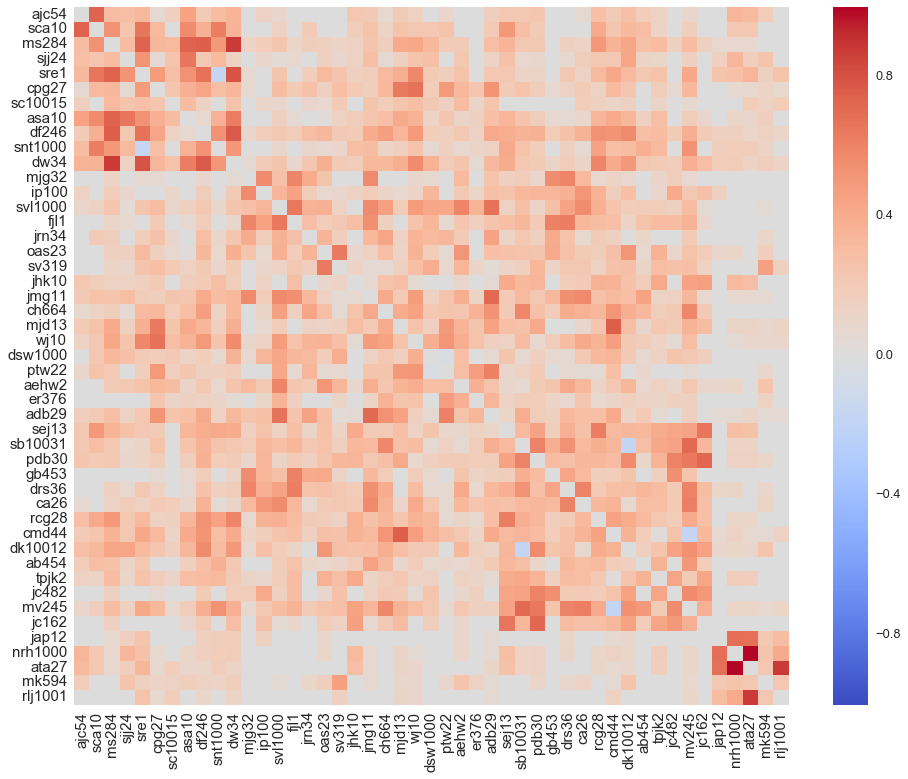
\includegraphics[width=\textwidth]{Analysis/Recommending_Mat.png}
    \caption[Recommended Collaboration Matrix]{High values (Deep red) indicate authors that have similar research but for which there is little evidence of collaboration on published works. Values $\sim$ 0 (grey/white) are where authors are neither similar nor collaborate, or are similar and collaborate closely. Values towards -1, (Blue) indicate authors that are collaborate but do share similar research (not strongly observed, as expected. High negative values would be somewhat paradoxical.) }
    \label{fig:RECOMM_MAT}

\end{figure} 
\end{center}
This final piece of the analysis section illustrates how the framework developed over the research project reveals where it might be profitable for authors to collaborate. Returning to the Centre for Atmospheric Science, which was highlighted as a tight, separate research community, it can be seen that there are recommendations for greater collaboration between particular authors within the Centre. Table \ref{tab:topcollabs} shows the top 20 scores in the Recommended Collaboration Matrix, where there is stronger evidence to suggest these author pairs should collaborate but little evidence that they are collaborating.

\begin{table}[H]
\centering
\caption{Community 275}
\label{tab:topcollabs}
\begin{tabular}{||c|Z|Z|Z||}
\hline
Rank & Author CRSID & Author CRSID & Recommended Collaboration Matrix Score \\
\hline
1 & ata27 & nrh1000 & 1.000 \\ 
2 & dw34 & df246 & 0.916 \\ 
3 & dw34 & ms284 & 0.875 \\ 
4 & rlj1001 & ata27 & 0.875 \\ 
5 & dw34 & sre1 & 0.795 \\ 
6 & adb29 & ptw22 & 0.765 \\ 
7 & cmd44 & mjd13 & 0.757 \\ 
8 & df246 & ms284 & 0.755 \\ 
9 & ca26 & drs36 & 0.753 \\ 
10 & sca10 & ajc54 & 0.737 \\ 
11 & sre1 & ms284 & 0.737 \\ 
12 & adb29 & wj10 & 0.736 \\ 
13 & mv245 & pdb30 & 0.731 \\ 
14 & asa10 & ms284 & 0.730 \\ 
15 & jc162 & pdb30 & 0.724 \\ 
16 & adb29 & jmg11 & 0.714 \\ 
17 & mv245 & sb10031 & 0.713 \\ 
18 & ca26 & fjl1 & 0.708 \\ 
19 & df246 & sre1 & 0.679 \\ 
20 & adb29 & svl1000 & 0.676 \\ 
\hline
\end{tabular}
\end{table}

The matrix row for a particular staff member (Professor Goodman) is plotted below by way of example of what the model considers a staff member's recommendations to be.
\begin{center}
\begin{figure}[H]
  \centering
  \textbf{Recommended Collaboration Scores for Particular Staff Member, Professor Goodman}
    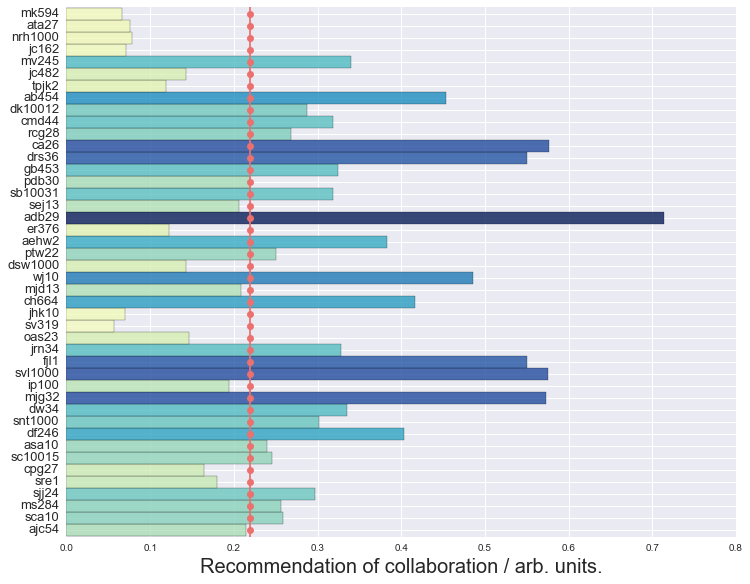
\includegraphics[width=\textwidth]{Analysis/jmg_dots_line.png}
    \caption[Recommended Collaboration Scores for Particular Staff Member]{Recommendations for a particular staff member from the recommendation matrix, plotted in bar form, (Professor Goodman). (Bars very close to zero have been removed). Large values (Long bars, deeper blue) indicate the author publishes in many similar communities to Professor Goodman, but little evidence was found of collaboration, thus the recommendation to collaborate. The vertical line indicates the \emph{mean} value in the Recommended Collaboration Matrix. Bars breaking through the line to the right are higher than the mean, and thus are where new collaborations should be considered.}
    \label{fig:RECOMM_BAR}
\end{figure} 
\end{center}
The aim is that these maps and plots may trigger new, constructive debate and promote effective collaboration in the department. The analyses presented in this section are not exhaustive, and there is potential for more fruitful insights to be found. Please see \S\ref{sec:RECOMMENDATIONS}. It should also be noted that the evidence for collaboration is from quite a small sample, and the collaboration metric could be improved by considering other factors than just co-authorship. It is also possible some co-authorships could not be resolved due to data incompatibilities between databases.

